% Section 3.3. Translated paragraph by paragraph from the updated Word source.
\subsection{Full-Duplex Speech Interaction}\label{sec:full-duplex}

% Word paragraph 1
Full-duplex speech interaction extends half-duplex turn-based interaction to concurrent behaviors such as simultaneous listening and speaking, interruption and floor-taking, and backchanneling. Conversational timing control consequently becomes central to interaction intelligence. According to the depth of coupling between timing control and the language-model backbone, this section distinguishes three paradigms: module-level external control, semi-embedded semantic assistance, and native dynamic interaction. These paradigms represent progressively tighter coupling between timing control and the backbone. Their mechanisms are examined in terms of timing-decision formation and streaming execution (Figure~\ref{fig:fullduplex}).

% Word paragraph 3; the original figure is preserved.
\begin{figure}[!htbp]
\centering
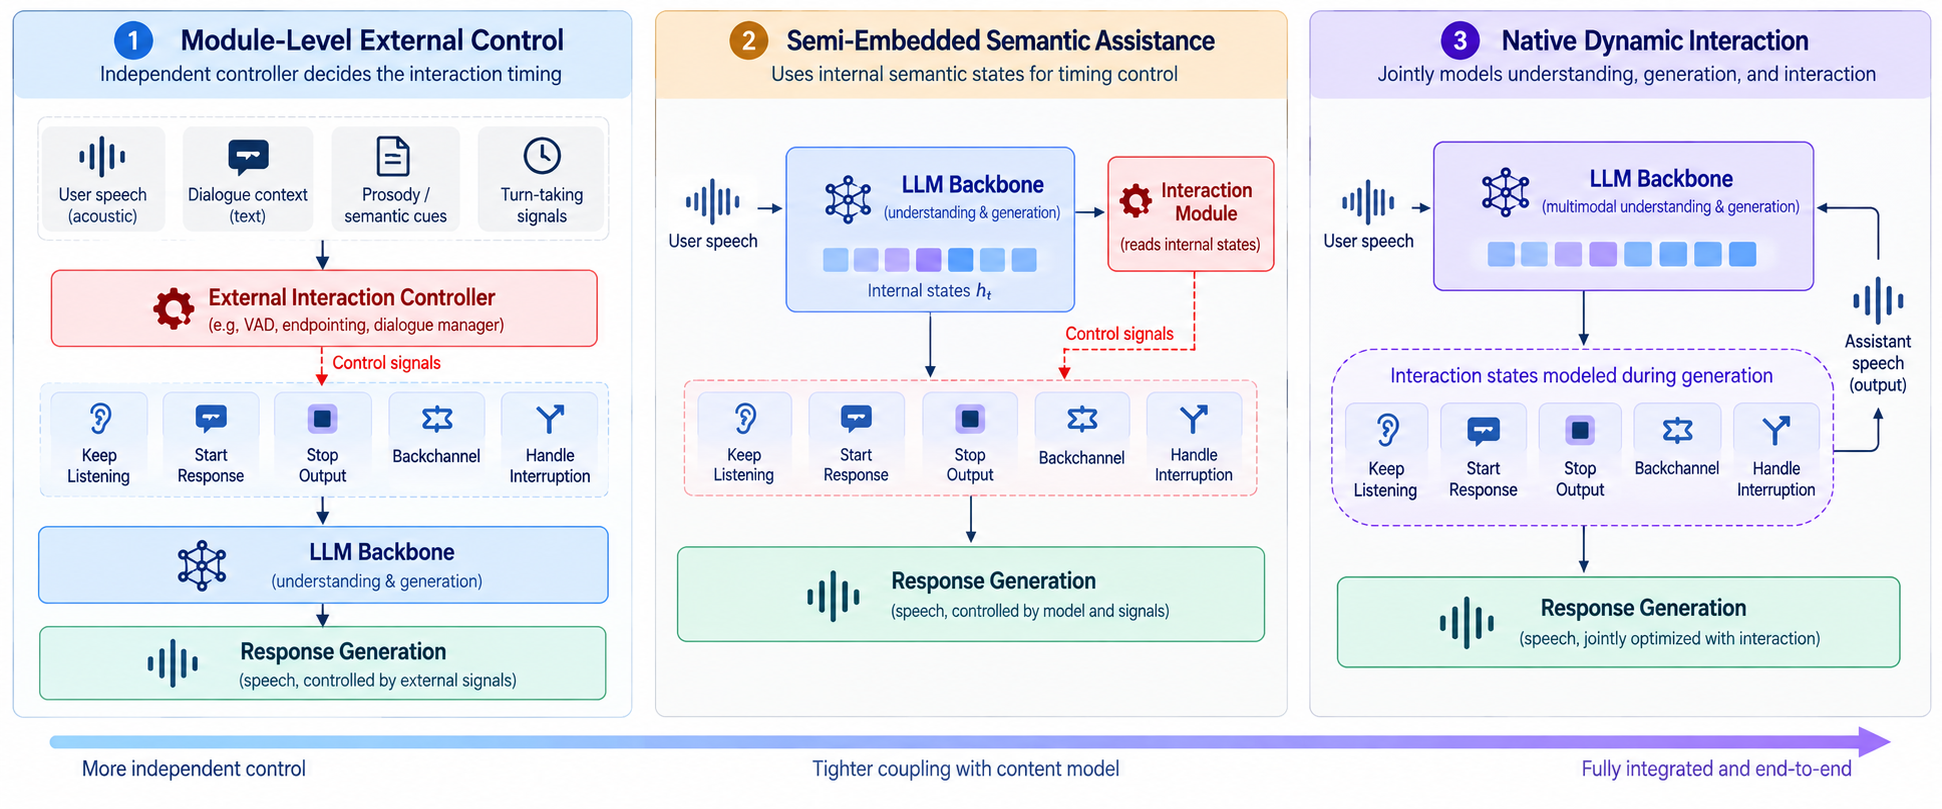
\includegraphics[width=\linewidth]{figures/fullduplex}
\caption{Three paradigms for coupling conversational timing control with the language-model backbone. From left to right: module-level external control, semi-embedded semantic assistance, and native dynamic interaction. The figure illustrates the control paths and execution interfaces of the three paradigms.}
\label{fig:fullduplex}
\end{figure}

% Word paragraph 4
\subsubsection{Module-Level External Control}\label{sec:fd-external}

% Word paragraph 5
Module-level external control places conversational timing control outside the language-model backbone. Independent external components, such as voice activity detection, endpoint detection, and dialogue management, make full-duplex interaction decisions and regulate input admission and response execution through explicit interfaces. Within this paradigm, the language model generates replies from admitted input and dialogue context, while an external controller schedules turn transitions, interruption handling, and backchannel initiation. This organization allows existing half-duplex backends to be reused when extending a system to full-duplex interaction.

% Word paragraphs 6--7
\paragraph{Evidence and state prediction for timing control.}
External timing control combines evidence of utterance completion with conditions for taking the floor. Dialogue context provides evidence of semantic completion, which TurnGPT uses to predict turn endings~\citep{DBLP:journals/corr/abs-2010-10874}. RC-TurnGPT adds a candidate response, extending the judgment to whether taking the floor is appropriate~\citep{DBLP:conf/acl/JiangES23}. Speech timing provides complementary evidence about how vocal activity may unfold: VAP projects future voice activity~\citep{DBLP:conf/interspeech/EkstedtS22}, while Next-Turn uses time-to-next-speech-onset supervision for streaming endpoint detection~\citep{DBLP:journals/corr/abs-2606-18094}. To guide execution, the controller maps these cues to states or actions. Joint modeling connects perception with state estimation. FlexDuo combines audio, dialogue history, and the previous state to predict Speak, Listen, and Idle actions~\citep{DBLP:journals/corr/abs-2502-13472}; SoulX-Duplug jointly predicts streaming ASR text and user states within an independent controller~\citep{arXiv:2603.14877}. Separate detection instead assigns individual control conditions to specialized prediction tasks. FireRedChat separates target-speaker activity from semantic end-of-turn detection, providing distinct triggers for playback pausing and complete-input submission~\citep{DBLP:journals/corr/abs-2509-06502}. SID focuses on semantic interruption intent to inform whether output should stop~\citep{DBLP:journals/corr/abs-2603-24144}. These designs allow the controller to predict a joint state directly or combine intermediate judgments.

% Word paragraphs 8--9. The repeated FireRedChat/X-Talk/SID passage is merged.
\paragraph{Streaming execution and response coordination.}
Timing predictions become interaction behavior through input admission and output scheduling. Input admission first determines which observations reach the response-generation backend. FlexDuo predicts actions over sliding audio windows, buffering relevant speech in Listen and filtering irrelevant input in Idle; SoulX-Duplug passes transcription results and state estimates to the generation pipeline. As new input arrives, evidence becomes clearer over time, so playback pausing and generation cancellation often proceed in stages. FireRedChat first pauses playback upon detecting target-speaker activity, then submits the input after semantic completion. X-Talk distributes these responsibilities between the client, which pauses immediately, and the server, which verifies the interruption before canceling inference and synthesis or resuming playback~\citep{DBLP:journals/corr/abs-2512-18706}. SID smooths successive predictions and requires repeated interruption judgments before issuing a stop command, limiting the effect of transient errors. These confirmation policies balance responsiveness against false triggering. Changes to output also require dialogue history to reflect what was actually played. The TurnGPT/VAP robot integration retains only the played response in shared history~\citep{DBLP:journals/corr/abs-2501-08946}, allowing subsequent generation to continue from what the user has heard. Input admission, output control, and history updates together maintain consistency during streaming interaction.

% Word paragraph 10
Module-level external control links timing prediction and response generation through explicit interfaces. Its principal technical differences concern decision evidence, state representations, and action-triggering conditions. Semi-embedded semantic assistance further uses the language model's internal representations to form timing decisions, establishing a more direct connection between interaction control and content generation.

% Word paragraph 11
\subsubsection{Semi-Embedded Semantic Assistance}\label{sec:fd-semi}

% Word paragraph 12
Semi-embedded semantic assistance connects conversational timing control with the language model at the representation level. Typical approaches predict interaction states from the model's contextual hidden representations, then coordinate response initiation, output stopping, and backchannel triggering through a relatively separate control path. The language model thus provides both response content and semantic evidence for timing judgments, while explicit prediction mechanisms and runtime scheduling trigger the resulting control actions.

% Word paragraphs 13--14
\paragraph{Timing prediction and learning from shared representations.}
Semi-embedded methods draw on the content backbone's internal semantic representations, with different choices of state readout and prediction targets. Freeze-Omni reads the language model's final-layer hidden states at input speech-chunk boundaries to distinguish continued input reception, completed speech requiring interruption, and completed speech without interruption~\citep{DBLP:journals/corr/abs-2411-00774}. MinMo uses a Transformer--softmax predictor over the content backbone's hidden representations to determine when to initiate a response or stop output~\citep{DBLP:journals/corr/abs-2501-06282}. BC head reads the temporal Transformer states of a full-duplex host model specifically to predict assistant backchannel onset~\citep{DBLP:journals/corr/abs-2609-29418}. Training strategies further determine how timing control uses these representations. Freeze-Omni optimizes state-prediction and text-generation objectives while keeping the content backbone frozen. MinMo trains its timing predictor in a dedicated full-duplex alignment stage. BC head uses focal loss for sparse backchannel-onset labels and adapts the host backbone through LoRA in its PersonaPlex configuration. VITA provides a boundary case: input admission is determined by model-generated query-state tokens, without a separate hidden-state prediction head~\citep{DBLP:journals/corr/abs-2408-05211}. These designs use the language model's existing semantic understanding while learning specific interaction behaviors through different supervision targets and parameter-adaptation strategies.

% Word paragraphs 15--16
\paragraph{State readout and streaming response control.}
Shared semantic representations provide evidence for timing judgments, while state readout and scheduling determine when predictions can affect output. Freeze-Omni reads classification results at input-chunk boundaries and uses session-level caches to manage subsequent input reception and response generation~\citep{DBLP:journals/corr/abs-2411-00774}. MinMo uses the output of a separate predictor to initiate a response or stop the current speech output~\citep{DBLP:journals/corr/abs-2501-06282}. BC head predicts backchannel-onset probabilities frame by frame and forces a \texttt{[BC]} marker when a preset threshold is exceeded; the host then generates the backchannel's wording and speech autoregressively~\citep{DBLP:journals/corr/abs-2609-29418}. These mechanisms translate timing predictions into execution actions through explicit control interfaces, with different state-update granularities, triggering conditions, and interventions in generation. VITA follows a different execution path: once a listening instance confirms a valid query, the listening and generation instances exchange roles, translating a semantic state judgment into a change of execution ownership~\citep{DBLP:journals/corr/abs-2408-05211}. Chunk-level state classification, framewise onset prediction, and dual-instance scheduling therefore impose different constraints on decision-update frequency, action commitment, and response continuity, despite their shared use of semantic understanding.

% Word paragraph 17
Semi-embedded semantic assistance strengthens the semantic basis of timing prediction through shared content representations while retaining relatively separate state-estimation and execution-control mechanisms. It combines the model's understanding capabilities with explicit interaction control. Native dynamic interaction further incorporates timing behavior into the language model's ongoing generation, allowing response content and timing decisions to be updated together as new input arrives.

% Word paragraph 18
\subsubsection{Native Dynamic Interaction}\label{sec:fd-native}

% Word paragraph 19
Native dynamic interaction incorporates conversational timing control into the language-model backbone's ongoing generative process. It jointly models response content, vocal activity, and control over continuously updated input, determining behaviors such as speaking, listening, pausing, interruption, and backchanneling. Timing decisions are generated together with response content, with reduced reliance on separate state-prediction modules.

% Word paragraphs 20--21
\paragraph{Joint representation and learning of content and timing.}
Native dynamic interaction incorporates pauses, overlap, and turn transitions into ongoing prediction. The main difference among approaches lies in how they organize the speech and interaction states of both participants. Parallel-stream modeling aligns separate semantic channels for each speaker, allowing the model to learn vocal activity and its temporal dependencies jointly. dGSLM connects the two speech streams through cross-attention~\citep{DBLP:journals/tacl/NguyenKCAHETASM23}, and NTPP predicts aligned tokens for both channels using pairwise causal masking~\citep{DBLP:journals/corr/abs-2506-00975}. Moshi also models assistant text alongside the user and assistant speech streams~\citep{DBLP:journals/corr/abs-2410-00037}. Flattened sequence modeling places modalities and interaction states in a single autoregressive sequence. OmniFlatten flattens chunks of user speech, assistant text, and assistant speech into this sequence and uses silence tokens to represent waiting~\citep{DBLP:conf/acl/ZhangCDCWZLYTDZ25}. BayLing-Duplex combines state tokens with timing preference learning to improve speaking and stopping decisions~\citep{DBLP:journals/corr/abs-2606-14528}. In a cascaded architecture, DuplexCascade serializes ASR micro-turns and generates control actions with the content LLM~\citep{DBLP:journals/corr/abs-2603-09180}. Alternating chunk schedules organize updates in both directions and response generation into time windows. SyncLLM predicts concurrent user speech chunks and later replaces them with observed speech~\citep{DBLP:conf/emnlp/VeluriPYGG24}, while AdaptDuplex learns to predict interaction behavior and the duration of the next window to adjust how often it updates~\citep{DBLP:journals/corr/abs-2609-29217}. These three designs emphasize, respectively, preserving information from concurrent speech, representing content and states in a common sequence, and controlling the timing of input and output updates.

% Required packages: booktabs, array, tabularx, caption.

\begin{table*}[!tp]
\centering
\captionsetup{font=footnotesize,labelfont=bf,skip=4pt}

\caption[Overview of full-duplex speech interaction systems and related methods]{
Overview of full-duplex speech interaction systems and related methods.
Systems are grouped by the depth of coupling between conversational timing
control and the language-model backbone, then ordered by speech architecture
(modular, Thinker--Talker, or native end-to-end).
VAD denotes voice activity detection, EoT end of turn, ASR automatic speech
recognition, TTS text-to-speech, and TAIL Time-Aligned Interleaving.
IRQ and \texttt{[BC]} mark interruption and backchannel onset, respectively.
}
\label{tab:fd-overview}

\scriptsize
\setlength{\tabcolsep}{2.5pt}
\setlength{\extrarowheight}{0pt}
\renewcommand{\arraystretch}{1.15}

\begin{tabularx}{\linewidth}{@{}
    >{\raggedright\arraybackslash}p{0.25\linewidth}
    >{\raggedright\arraybackslash}p{0.115\linewidth}
    >{\raggedright\arraybackslash}p{0.18\linewidth}
    >{\raggedright\arraybackslash\setlength{\baselineskip}{9.5pt}}X
@{}}
\toprule
\textbf{System / Work}
& \textbf{Architecture}
& \textbf{Input / Output}
& \textbf{Highlight} \\
\midrule

\multicolumn{4}{@{}l}{
    \textit{Module-Level External Control: Independent controllers make timing decisions}
} \\
\midrule

FireRedChat~\citep{DBLP:journals/corr/abs-2509-06502}
& Modular
& Speech / Text, Speech
& Target-speaker VAD pauses audio. Semantic EoT submits input \\

X-Talk~\citep{DBLP:journals/corr/abs-2512-18706}
& Modular
& Speech / Text, Speech
& Client pauses. Backend verifies before canceling or resuming \\

SoulX-Duplug~\citep{arXiv:2603.14877}
& Modular
& Speech / Speech
& Joint streaming ASR/state prediction controls LLM--TTS \\

FlexDuo (GLM-4-Voice)~\citep{DBLP:journals/corr/abs-2502-13472}
& Native
& Speech / Speech
& Independent Speak/Listen/Idle prediction; input filtering and buffering \\

\midrule
\multicolumn{4}{@{}l}{
    \textit{Semi-Embedded Semantic Assistance: Explicit timing prediction from shared backbone representations}
} \\
\midrule

VITA~\citep{DBLP:journals/corr/abs-2408-05211}
& Modular
& Text, Audio, Image, Video / Text, Speech
& Query-state tokens identify valid input; dual-instance switching and external TTS \\

Freeze-Omni~\citep{DBLP:journals/corr/abs-2411-00774}
& Thinker--Talker
& Text, Speech / Text, Speech
& Chunk-end hidden-state classification; frozen backbone and cache-based response scheduling \\

MinMo~\citep{DBLP:journals/corr/abs-2501-06282}
& Thinker--Talker
& Text, Audio / Text, Speech
& Transformer--softmax maps backbone states to start/stop \\

BC head (PersonaPlex/F-Actor)~\citep{DBLP:journals/corr/abs-2609-29418}
& Native
& Speech / Speech
& Hidden-state backchannel-onset prediction; a threshold triggers forced \texttt{[BC]} decoding \\

\midrule
\multicolumn{4}{@{}l}{
    \textit{Native Dynamic Interaction: Joint modeling of response content and timing during continuous generation}
} \\
\midrule

DuplexCascade~\citep{DBLP:journals/corr/abs-2603-09180}
& Modular
& Speech / Text, Speech
& Continuous ASR micro-turn input; LLM-generated wait/respond/backchannel actions \\

CT-Duplex~\citep{DBLP:journals/corr/abs-2510-05150}
& Thinker--Talker
& Speech / Text, Speech
& Causal reasoning while listening. States guide speech decoding \\

SALMONN-omni~\citep{DBLP:journals/corr/abs-2505-17060}
& Thinker--Talker
& Audio / Text, Speech
& Listening/speaking states generated with text; output embeddings condition streaming synthesis \\

MiniCPM-o 4.5~\citep{DBLP:journals/corr/abs-2604-27393}
& Thinker--Talker
& Text, Audio, Image, Video / Text, Speech
& Omni-Flow aligns input/output; TAIL bounds text-ahead using playback progress \\

DuplexOmni~\citep{DBLP:journals/corr/abs-2606-09186}
& Thinker--Talker
& Audio, Video / Text, Speech
& Time-sliced interaction; asynchronous integration of background reasoning and tool results \\

Realtime-Venus (Audio/Omni)~\citep{DBLP:journals/corr/abs-2609-13814}
& Thinker--Talker
& Text, Audio, Image, Video / Text, Speech
& Shared causal timeline for perception, responses, and control; asynchronous task delegation \\

AdaptDuplex~\citep{DBLP:journals/corr/abs-2609-29217}
& Thinker--Talker
& Speech / Text, Speech
& Behavior and window-duration tokens; bounded text-ahead and a turn-local queue \\

D2 (Qwen3-Omni/LLaMA-Omni 2)~\citep{arXiv:2610.17124}
& Thinker--Talker
& Audio / Text, Speech
& Encoder distillation and duplex fine-tuning; each chunk uses new input and delayed self-audio \\

dGSLM~\citep{DBLP:journals/tacl/NguyenKCAHETASM23}
& Native
& Speech / Speech
& Dual-channel continuation; cross-attention jointly predicts speech units and durations \\

LSLM~\citep{DBLP:conf/aaai/MaSDC0WW025}
& Native
& Text, Speech / Speech
& Continuous listening features condition speech decoding; an IRQ token stops output \\

Moshi~\citep{DBLP:journals/corr/abs-2410-00037}
& Native
& Speech / Text, Speech
& Aligned user/assistant streams; temporal modeling and within-frame codebook prediction \\

SyncLLM~\citep{DBLP:conf/emnlp/VeluriPYGG24}
& Native
& Speech / Speech
& Simulated bidirectional interaction; predicted concurrent user chunks replaced by observations \\

OmniFlatten~\citep{DBLP:conf/acl/ZhangCDCWZLYTDZ25}
& Native
& Text, Speech / Text, Speech
& Flattened speech/text with silence tokens for waiting \\

Voila-autonomous~\citep{DBLP:journals/corr/abs-2505-02707}
& Native
& Text, Speech / Text, Speech
& Dual-stream embedding fusion; hierarchical semantic/acoustic generation and voice conditioning \\

SALM-Duplex~\citep{DBLP:journals/corr/abs-2505-15670}
& Native
& Speech / Text, Speech
& Continuous user features fused with assistant streams; parallel text/codebook prediction \\

NTPP~\citep{DBLP:journals/corr/abs-2506-00975}
& Native
& Speech / Speech
& Dual-channel continuation; pairwise causal masking jointly predicts aligned speech tokens \\

TurnGuide~\citep{DBLP:journals/corr/abs-2508-07375}
& Native
& Speech / Text, Speech
& Dynamic turn splits with aligned text--speech interleaving \\

FLM-Audio~\citep{DBLP:journals/corr/abs-2509-02521}
& Native
& Text, Speech / Text, Speech
& Contiguous monologues and waiting intervals; dual text/speech training \\

Fun-Audio-Chat-Duplex~\citep{DBLP:journals/corr/abs-2512-20156}
& Native
& Text, Audio / Text, Speech
& Parallel user/assistant speech input; low-rate backbone and higher-rate speech refinement \\

PersonaPlex~\citep{DBLP:journals/corr/abs-2602-06053}
& Native
& Text, Speech / Text, Speech
& Moshi-style dual-stream generation; text role prompts and audio voice prompts \\

F-Actor~\citep{DBLP:journals/corr/abs-2601-11329}
& Native
& Text, Speech / Text, Speech
& Instruction-controlled initiation/backchannels/interruption; original codec constrains streaming inference \\

Raon-SpeechChat~\citep{DBLP:journals/corr/abs-2605-23912}
& Native
& Text, Speech / Text, Speech
& Causal input encoding and interleaved generation; silence/onset/backchannel tokens \\

BayLing-Duplex~\citep{DBLP:journals/corr/abs-2606-14528}
& Native
& Speech / Text, Speech
& Causal chunk offsets and timing preferences at fixed content \\

Lychee-FD~\citep{DBLP:conf/acl/LiuZLTJCZMXHHLZ26}
& Native
& Speech / Text, Speech
& Deep semantic/acoustic split with a semantic alignment channel \\

MultiTalk~\citep{DBLP:journals/corr/abs-2609-36903}
& Native
& Speech / Text, Speech
& Moshi-style generation extended to long, multi-party bilingual dialogue and addressee selection \\

\bottomrule
\end{tabularx}
\end{table*}

\par\smallskip
\noindent\begin{minipage}{\linewidth}
\ifdefined\TakeawayBox\else
  \newenvironment{TakeawayBox}[1]
    {\small\noindent\textbf{#1}\par\smallskip}
    {\par}
\fi
\end{minipage}\par

% Word paragraphs 22--23
\paragraph{Causal input updates and generation--playback synchronization.}
Continuous generation requires timely access to new input so that subsequent responses can adapt as the dialogue unfolds. Through streaming-encoder distillation and full-duplex fine-tuning, D2 conditions output chunks on incoming user speech and delayed self-audio feedback~\citep{arXiv:2610.17124}. Once input enters generation, the update schedule determines opportunities to respond: MiniCPM-o 4.5's Omni-Flow advances input and output within aligned time windows~\citep{DBLP:journals/corr/abs-2604-27393}, while AdaptDuplex learns the next window's duration to adjust update granularity~\citep{DBLP:journals/corr/abs-2609-29217}. When interaction involves lengthy reasoning or tool tasks, DuplexOmni~\citep{DBLP:journals/corr/abs-2606-09186} and Realtime-Venus~\citep{DBLP:journals/corr/abs-2609-13814} use asynchronous execution to coordinate background computation with ongoing listening and speaking. These schedules must also track playback so that new decisions can promptly affect audible output. MiniCPM-o 4.5's TAIL limits textual lead according to playback progress, while AdaptDuplex likewise bounds text-ahead and manages speech-generation conditions through a turn-local queue. Input updates and playback synchronization jointly determine how readily a system can revise unplayed responses in light of new information.

% Word paragraph 24
Learning timing behavior within continuous generation allows responses and vocal activity to adapt to new input. Further development can build on coordination across timescales, integrating reasoning, tool use, and environmental perception while maintaining continuous listening and speaking. This would allow users to supply information, revise goals, and redirect interaction throughout task execution.

\begin{TakeawayBox}{Takeaways: Full-Duplex Speech Interaction}
Full-duplex interaction relies on pauses, overlapping speech, and backchannels
to coordinate participation. Existing approaches range from external
module-level control to semi-embedded semantic assistance and native dynamic
interaction. These approaches enable systems to adapt response timing and
content as users speak, interrupt, or revise their intentions. Coordinating
when to speak and what to say is key to natural full-duplex interaction.
\end{TakeawayBox}

% The overview float includes the takeaway below the table.

